\documentclass{standalone}
\usepackage{pgfplots}
\pgfplotsset{soldot/.style={color=black,only marks,mark=*},
             holdot/.style={color=black,fill=white,only marks,mark=*},
             compat=1.12}
\begin{document}
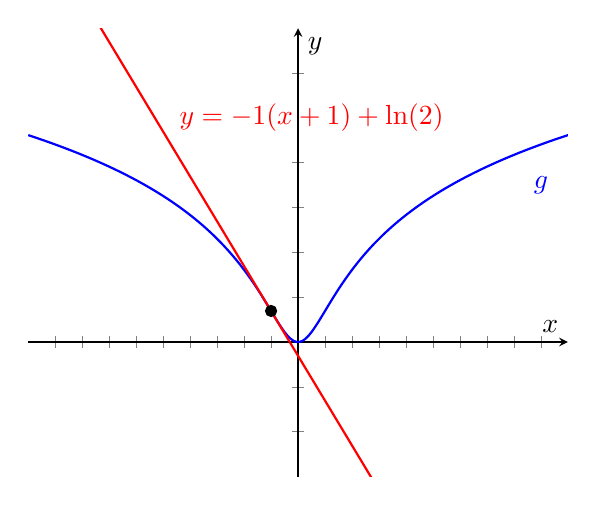
\begin{tikzpicture}
\begin{axis}[
 axis lines=middle,
 %ticklabel style={fill=blue!5!white},
 xmin=-10,xmax=10,
 ymin=-3,ymax=7,
 xtick={-9,...,1,2,3,4,5,6,7,...,9},xticklabels={},
 ytick={-2,...,1,2,3,4,6},yticklabels={},        %<--
% minor tick = {-5,-3,...,5}, %<--
 xlabel=\(x\),ylabel=\(y\),
 samples=200]

\addplot[domain=-10:12,thick,blue] {ln(x^2+1)};

\addplot[domain=-10:12,thick,red] {-1*(x+1)+ln(2)};

\draw [blue] (axis cs:9,3.5)  node [] {$g$};
\draw [red] (axis cs:0.5,5)  node [] {$y=-1(x+1)+\ln(2)$};
\addplot[soldot] coordinates{(-1,.6931)};

\end{axis}
\end{tikzpicture}
\end{document}